 % !TeX spellcheck = en_US
\documentclass[12pt]{article}
\usepackage{amssymb }
\usepackage{amsmath }
\usepackage{graphicx}


%opening
\title{Basic Mathematics for Biologists}
\author{Alberto Marin Sanguino}

\begin{document}

\maketitle

\begin{abstract}

\end{abstract}

\section{Ordinary differential equations}

A differential equation is an equality involving one or more unknowns ($x$, $y$, $z$,\dots) and their derivatives. Since our unknowns have derivatives, they are not just numbers like in regular -- a.k.a. algebraic -- equations. Our unknowns are functions or, more accurately, families of functions. We can make this explicit by writing our unknowns as $x(t)$, $y(t)$, $z(t)$,\dots thus sacrificing brevity for the sake of clarity. In the text that follows, very little effort will be made to mantain consistency between these two notations and we will wantonly switch between both. Live with it.

Among all differential equations, we will be interested in the simpler type. Ordinary differential equations (ODEs) are those that do not involve partial derivatives. Our functions will only have one independent variable that almost always will be time. Moreover, we will start with linear equations.

Linear equations are those where different unknowns and their derivatives are only combined linearly. Some examples of linear equations are:

\begin{align}
	\frac{dx}{dt} \: = \: &  a \, x	\\
	\frac{dx}{dt} + \frac{dy}{dt}\: = \: &  0 \\
	\frac{dx}{dt} \: = \: &  a \, x + b \, y
\end{align}

while the following equations are not linear:

\begin{align}
	\frac{dx}{dt} \: = \: &  x^2	\\
	\frac{dx}{dt} + \frac{dy}{dt}\: = \: &  x \, y \\
	\frac{dx}{dt} \: = \: &  \sin x 
\end{align}

Keep in mind that the linearity requirement only applies to the unknowns and not to the independent variable. The following equations are all linear


\begin{align}
	\frac{dx}{dt} \: = \: &  t^2 \, x	\\
	\frac{dx}{dt} + \frac{dy}{dt}\: = \: &  \sin t \\
	\frac{dx}{dt} \: = \: &  t \, x + t^2 \, y
\end{align}

In these equations, the coefficients that multiply our unknowns just happen to be functions of time. A linear equation can have coefficients that depend on time and also have time-dependent independent terms. In general, we will not concern ourselves with such systems.

\section{Linear equations}

Solving differential equations is very challenging, that's why we will try to avoid it whenever possible. In fact, we are only going to solve one differential equation during the whole course. We will solve this equation in two versions: with on variable and with several variables.

\subsection{Solving the linear equation with one variable}

Lets start with the simplest possible case, which also happens to describe a fundamental biological process: exponential growth.

\begin{equation}
	\label{odexp}
	\frac{dx}{dt} = \mu \, x
\end{equation}

Which can be read as: ``the rate of increase of a population $x$ is proportional to its own size.'' This equation is easy to solve because we can separate the variables:


\begin{equation}
	\frac{dx}{x} = \mu \, dt
\end{equation}

and integrate

\begin{equation}
	\int \frac{dx}{x} = \mu \, \int  dt
\end{equation}

\begin{equation}
	\ln{x} = \mu \, t + C
\end{equation}

Since $C$ is an arbitrary constant, we can define it in terms of another constant $C= \ln{k}$ so:

\begin{equation}
	\ln{x} - \ln{k}  = \mu \, t 
\end{equation}

Applying the well known properties of logarithms listed in appendix \ref{logprop}

\begin{equation}
	\ln{\frac{x}{k}}   = \mu \, t 
\end{equation}

exponentiating both sides and rearranging

\begin{equation}
	x   = k \, e^{\mu \, t}
\end{equation}

This is the \emph{general solution} of the differential equation. It is a family of functions because we can generate infinite functions assigning different values to k. For every possible value of $k$ there is a \emph{particular solution} of the equation.

We are not normally interested in general solutions. General solutions are for mathematicians. We want the particular solution that fits some \emph{initial condition}, $x(0)$, often written $x_0$. For instance, we have a bacterial culture that starts with an optical density of 0.01. How do we find the right value for k?


\begin{equation}
x(0) = 0.01 \Rightarrow	 k \, e^{\mu \, 0} = 0.01 \Rightarrow	k=0.01 
\end{equation}

In general, we use the solution to the exponential equation as:

\begin{equation}
	x   = x_0 \, e^{\mu \, t}
\end{equation}

\subsection{Solving the linear equation with several variables}


Our simple linear equation can also have more that one variable:

\begin{align}
	\label{odenvar}
	\frac{dx_1}{dt} =& a_{1,1} \, x_1 + a_{1,2} \, x_2 \nonumber\\
	\frac{dx_2}{dt} =& a_{2,1} \, x_1 + a_{2,2} \, x_2
\end{align}

when dealing with several variables, it helps a lot to use vectors and matrices.

\begin{equation}
	\frac{d}{dt} \begin{pmatrix} x_1\\ x_2 \end{pmatrix} = \begin{pmatrix} a_{1,1} & a_{1,2}\\ a_{2,1} & a_{2,2} \end{pmatrix} \begin{pmatrix} x_1\\ x_2 \end{pmatrix}
\end{equation}

Thus, we can write any equation with n variables as:

\begin{equation}
	\label{odenvar_mat}
	\frac{d\mathbf{x}}{dt}  = \mathbf{A} \, \mathbf{x}
\end{equation}

Note that vectors and matrices are written in boldface.

Since the solution of the equation for one variable was an exponential, lets make the hypothesis that an exponential can also be a solution for this case. We assume

\begin{equation}
	\mathbf{x}= \mathbf{v} \, e^{\lambda \, t}
\end{equation}

Since $\mathbf{x}$ is a vector now, we multiply our exponential times a  vector of constants $\mathbf{v}$. We can test if this is a valid solution by substituting it into the equation, which gives:

\begin{equation}
	\frac{d}{dt} \left( \mathbf{v} \, e^{\lambda \, t} \right)  = \mathbf{A} \, \mathbf{v} \, e^{\lambda \, t} 
\end{equation}

On the left hand side, the vector of  constants can be taken out of the derivative so:

\begin{equation}
	\mathbf{v} \, \frac{d}{dt} \left(  e^{\lambda \, t} \right)  = \mathbf{A} \, \mathbf{v} \, e^{\lambda \, t} 
\end{equation}
 
 and
 
 \begin{equation}
 	\mathbf{v}   \lambda \, e^{\lambda \, t}   = \mathbf{A} \, \mathbf{v} \, e^{\lambda \, t} 
 \end{equation}
 
canceling out the exponentials:

\begin{equation}
\label{eigendefinition}
\mathbf{A} \, \mathbf{v}  = \lambda  \,	\mathbf{v}   
\end{equation}
 
So $\mathbf{x}=\mathbf{v} \, e^{\lambda \, t}$ will be a solution of the equation as long as $\lambda$ and $\mathbf{v}$ satisfy equation (\ref{eigendefinition}).

We can solve the equation and find all possible values of $\lambda$ by rearranging terms.

\begin{equation}
	\mathbf{A} \, \mathbf{v}  - \mathbf{I} \, \lambda  \,	\mathbf{v}   = 0
\end{equation}

note we have multiplied lambda by the identity matrix $\mathbf{I}$. This is a matrix of zeros everywhere except its main diagonal, which is occupied by ones. The identity matrix plays the same role as number one among scalars, it does not alter the matrices or vectors it multiplies. Now we can factor $\mathbf{v}$ out 

\begin{equation}
	\label{solve4eigenvec}
	\left( \mathbf{A}   - \mathbf{I} \, \lambda     \right) \, \mathbf{v} =  0
\end{equation}

This is an homogeneous system of equations with the components of $\mathbf{v}$ as unknowns. For the system to have a solution other than the trivial, $\mathbf{v}=\mathbf{0}$, the determinant of the parenthesis must satisfy:

\begin{equation}
	\left| \mathbf{A}   - \mathbf{I} \, \lambda     \right|  =  0
\end{equation}

This determinant is the Jacobian of the system and its expansion results in a $n-th$ degree equation in terms of lambda known as the characteristic equation of the system.

\begin{equation}
c_n \, \lambda^n +c_{n-1} \, \lambda^{n-1}  + \dots  + c_1 \, \lambda + c_0 = 0
\end{equation}

\section{Eigenvalues and eigenvectors} 

\subsection{real eigenvalues}
A matrix $\mathbf{A}$ with size $n \times n$ has n vectors $\mathbf{v_i}$ for $i = 1 \dots n$ called eigenvectors, and each eigenvector has an eigenvalue ($\lambda_i$) such that every pair of eigenvector and eigenvalue satisfy equation (\ref{eigendefinition}).
	
In order to understand the meaning of this and why eigenvector and eigenvalues are extremely important in applied mathematics, we have to think of the matrix product as an operation that transforms one vector into another. For instance, lets take the matrix
\begin{equation}
	\mathbf{A}  = \begin{pmatrix} -1 & -4\\ -3 & -2\end{pmatrix} 
\end{equation}

If we multiply $(1,2)$ times the matrix we obtain another vector:

\begin{equation}
	 \begin{pmatrix} -1 & -4\\ -3 & -2\end{pmatrix} \,  \begin{pmatrix} 1\\ 2\end{pmatrix}=\begin{pmatrix} -9 \\ -7\end{pmatrix}
\end{equation}

So matrix $\mathbf{A}$ transforms  (1,2) into  (-9,-7). Now if  we transform another vector:

\begin{equation}
	\begin{pmatrix} -1 & -4\\ -3 & -2\end{pmatrix} \,  \begin{pmatrix} 4\\ -3\end{pmatrix}=\begin{pmatrix} 8 \\ -6\end{pmatrix}
\end{equation}

In the previous case, the transformation changed the direction of our vector but now, vector (4,-3) was transformed into a stretched version of itself with double length. If we now transformed $(8,-6)$ using the matrix, we would obtain $(16,-12)$, which is again the same vector multiplied by two. So (4,-3) is an eigenvector of $\mathbf{A}$ and the corresponding eigenvalue is $\lambda=2$. Note that negative eigenvalues will change the sense of the vector but not its direction, as is the case with the second eigenvector of this matrix $(1,1)$.

\begin{equation}
	\begin{pmatrix} -1 & -4\\ -3 & -2\end{pmatrix} \,  \begin{pmatrix} 1\\ 1\end{pmatrix}=- \begin{pmatrix} 5 \\ 5\end{pmatrix}
\end{equation}

Obviously, the corresponding eigenvalue is $\lambda=-5$.

But how can we find out the eigenvectors and eigenvalues of a matrix other than by trial and error? First we get the eigenvalues by equating the Jacobian determinant to zero:

\begin{equation}
  \left|\begin{matrix} -1-\lambda & -4\\ -3 & -2-\lambda\end{matrix} \right| = 0
\end{equation}

we get the characteristic polynomial

\begin{equation}
	\lambda^2  +3 \,  \lambda  - 10 = 0
\end{equation}

A primary school problem we can solve:

\begin{equation}
	\lambda= \frac{-3 \pm \sqrt{9+40}}{2}
\end{equation}

with two solutions $\lambda_1=2$ and $\lambda_2=-5$. We have already seen that the eigenvector $\mathbf{v_1}$ for $\lambda_1$ is . Can we find the other one? We can go back to equation (\ref{eigendefinition}) or use the already factored out version in equation  (\ref{solve4eigenvec})

\begin{equation}
\begin{pmatrix} -1-\lambda & -4\\ -3 & -2-\lambda\end{pmatrix} \, \begin{pmatrix} v_x \\  v_y\end{pmatrix} = 0
\end{equation}

For the case $\lambda = 2$:

\begin{equation}
	\begin{pmatrix} -3 & -4\\ -3 & 0\end{pmatrix} \, \begin{pmatrix} v_x \\  v_y\end{pmatrix} = 0
\end{equation}

\begin{align*}
	-3 \, v_x - 4 \, v_y =& 0\\
	-3 \, v_y =& 0
\end{align*}

The second equation shows a very important property of eigenvectors, they are never unique. In this case, any value of $v_y$ will satisfy the second equation, so we can assign whatever we want. Now it is easy to see that v=(4,-3) cancels out the first equation. If we had just chosen $v_y=1$, then our eigenvector would have been $\mathbf{v}=\left( \frac{-4}{3}, 1 \right)$.

Now we can do the same for  $\lambda = -5$:

\begin{align*}
	4 \, v_x - 4 \, v_y =& 0\\
	- 3 \, v_x  + 3 \, v_y =& 0
\end{align*}

This is actually the same equation twice. It is easy to see that whenever $v_x=v_y$, both equations will be satisfied, so we can choose $\mathbf{v} = (1, 1)$.

\paragraph{Exercise:} Can you use equation (\ref{eigendefinition}) to show that given an eigenvector $\mathbf{v}$ and a constant $k$, any vector $k \, \mathbf{v}$ will also be an eigenvector?

\subsection{Complex eigenvalues}

Now lets analyze another matrix 

\begin{equation}
	\mathbf{A}  = \begin{pmatrix} 0 & -1\\ 1 & 0\end{pmatrix} 
\end{equation}

Characteristic polynomial

\begin{equation}
	\lambda^2 + 1 = 0
\end{equation}

The solutions to this equation are imaginary $\lambda_1 = i$ and $\lambda_1 = -i$.

Complex eigenvalues always come in conjugate pairs: $\lambda_1 = a + b\, i$,  $\lambda_2 = a - b\, i$. In the context of ODEs, The real parts of a complex eigenvalue determine the stability, just as real eigenvalues do, while the existence of imaginary parts involves the existence of oscillations. Note that imaginary eigenvalues can only appear for systems with two or more variables. This means that for a system to oscillate, it must have at least two variables.


\section{General solutions for linear equations}

So putting together all the eigenvecotrs of the system and the corresponding eigenvalues, we get the general solution for our equation with n variables:


\begin{equation}
	\label{odenvar_mat_sol}
	\mathbf{x}= c_1 \, \mathbf{v_1} \, e^{\lambda_1 \, t} + c_2 \, \mathbf{v_2} \, e^{\lambda_2 \, t} +  \dots + c_n \, \mathbf{v_n} \, e^{\lambda_n \, t}
\end{equation}

Where $c_1 \dots c_n$  are arbitrary constants, the ones that can be used to adjust initial values. Each vector $\mathbf{v_i}$ and its corresponding constant $\lambda_i$ are called eigenvector and eigenvalue respectively.


When the eigenvalues (and eigenvectors) are complex, the solutions described above will be complex. But we are not interested in complex solutions, since all our models have real variables. To see how complex eigenvalues cause oscillations in real solutions, lets see a combination of complex exponentials:

\begin{equation}
	x_1= c_1 e^{\left(  a + b\, i\right) \, t} + c_2 \,  e^{\left(  a + b\, i\right)\, t} = 
	c_1  \, e^{a \, t} \, e^{ i \, b \, t} + c_2 \,  e^{a \, t} \, e^{-i \, b \, t}
\end{equation}

factoring out the real exponential

\begin{equation}
x_1= e^{a \, t} \,  \left( c_1  \, e^{ i \, b \, t} + c_2 \,  e^{-i \, b \, t}\right)
\end{equation}

Using Euler's formula:

\begin{equation}
	\label{euler}
	e^{i \theta} = cos \theta + i \, \sin \theta
\end{equation}

\begin{equation}
	x_1= e^{a \, t} \,  \left( c_1  \, \left(  \cos{ b \, t} + i \, \sin{ b \, t} \right)+ c_2 \, \left( \cos{- b \, t} + i \, \sin{- b \, t} \right) \right)
\end{equation}

\begin{figure}
\begin{center}
	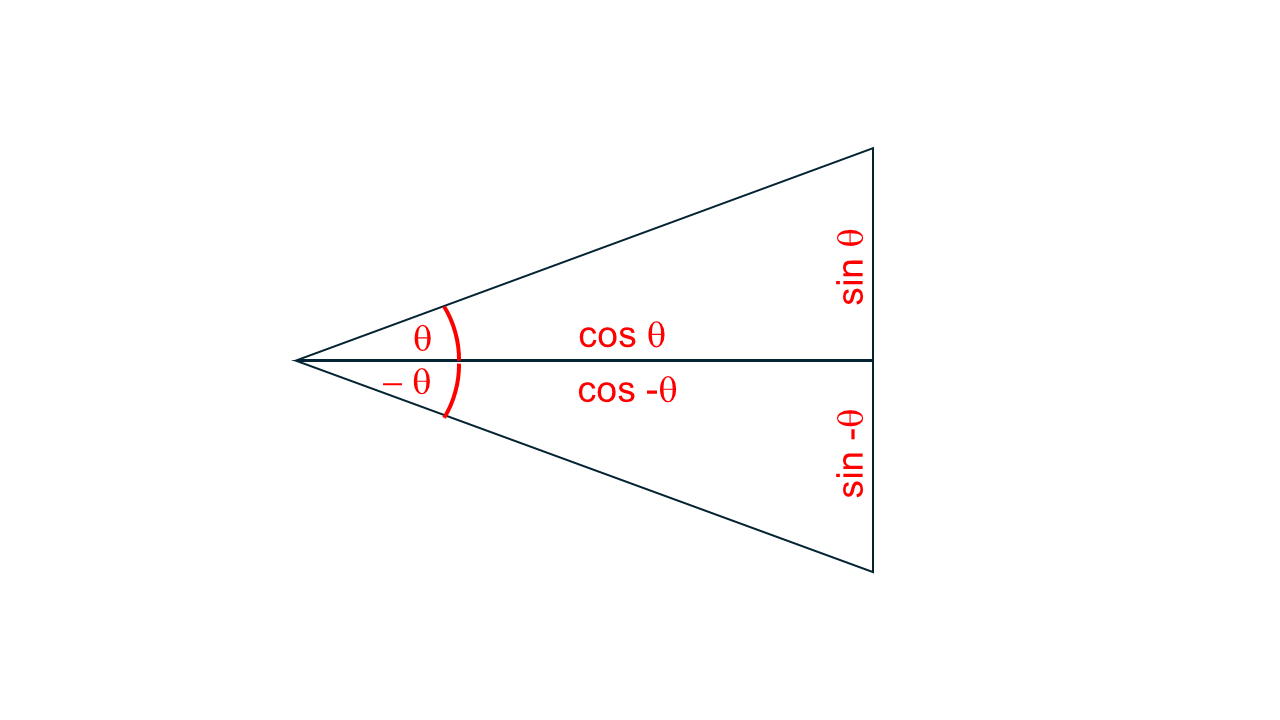
\includegraphics[width=\textwidth]{trigo}
\end{center}
\caption{Some basic trigonometric relations.}
\label{fig:trigo}
\end{figure}

As can be seen in  figure \ref{fig:trigo}, $- \sin{b \, t}=\sin{- b \, t}$ and $\cos{b \, t}=\cos{ - b \, t}$ so we can rearrange terms:

\begin{equation}
	x_1= e^{a \, t} \,  \left( c_1  \, \left(  \cos{ b \, t} + i \, \sin{ b \, t} \right)+ c_2 \, \left( \cos{ b \, t} - i \, \sin{ b \, t} \right) \right)
\end{equation}


\begin{equation}
	x_1=   \left( c_1+c_2\right) \, e^{a \, t} \, \cos{ b \, t}  + i \, \,\left( c_1-c_2 \right) \,e^{a \, t} \,   \sin{ b \, t}  
\end{equation}

Note that this solution has the form $x_1(t) = u(t) + i \, v(t)$ where both $u(t)$ and $v(t)$ are real functions. Moreover, these functions are linearly independent so a combination of both will be a proper general solution. By defining new arbitrary constants, we will get the general solution that includes al possible real solutions of the equation:

\begin{equation}
	x_1=   e^{a \, t} \,  \left(  A  \, \cos{ b \, t}  +  B  \,   \sin{ b \, t}  \right)
\end{equation}

So the real part of our solutions will be the product of an exponential and an oscillatory function. Moreover, the exponential depends only on the real part of the eigenvalue, $\operatorname{Re}(\lambda) = a$, while the oscillations depend on its imaginary part,  $\operatorname{Im}(\lambda) =b$ (see figure \ref{fig:cmplxeigen}). 

\begin{figure}
	\begin{center}
		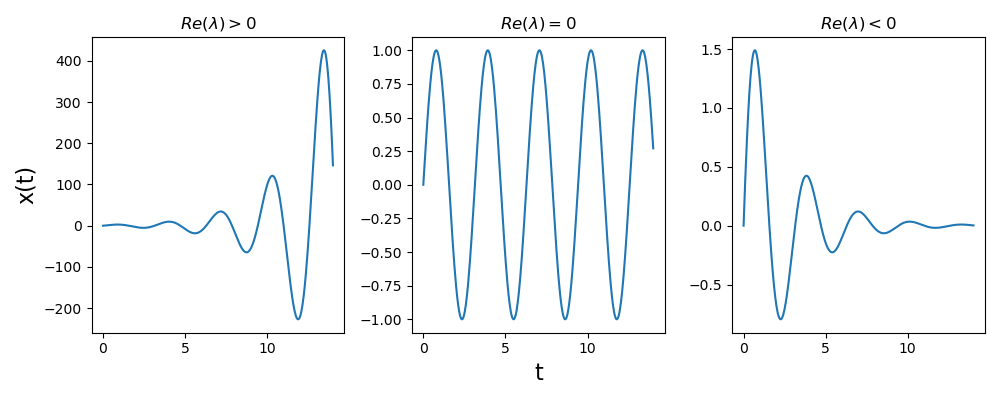
\includegraphics[width=\textwidth]{complex_eigen}
	\end{center}
	\caption{Overal behavior of solutions when eigenvalues are complex. The sign of $\operatorname{Re}(\lambda)$ determines stability and$\operatorname{Re}(\lambda)$ governs oscillations}
	\label{fig:cmplxeigen}
\end{figure}




\section{Differential equations of higher order}

\section{Plotting solutions}


\appendix
\section{Some properties of logarithms}
\label{logprop}
\begin{equation}
 \log{(a \, b)} =	\log{a} + \log{b} 
\end{equation}

\begin{equation}
	\log{(a / b)} =	\log{a} - \log{b} 
\end{equation}

\begin{equation}
	\log{x^a} =a \, \log{x} 
\end{equation}

\begin{equation}
	e^{\ln{x}} = x 
\end{equation}












\end{document}
